\documentclass[border=10pt]{standalone}

\usepackage{tikz}
\usepackage{tikzsymbols}
\usetikzlibrary{calc,patterns,shapes.geometric}

\def\centerarc[#1](#2)(#3:#4:#5){\draw[#1] ($(#2)+({#5*cos(#3)},{#5*sin(#3)})$) arc (#3:#4:#5);}

\begin{document}
	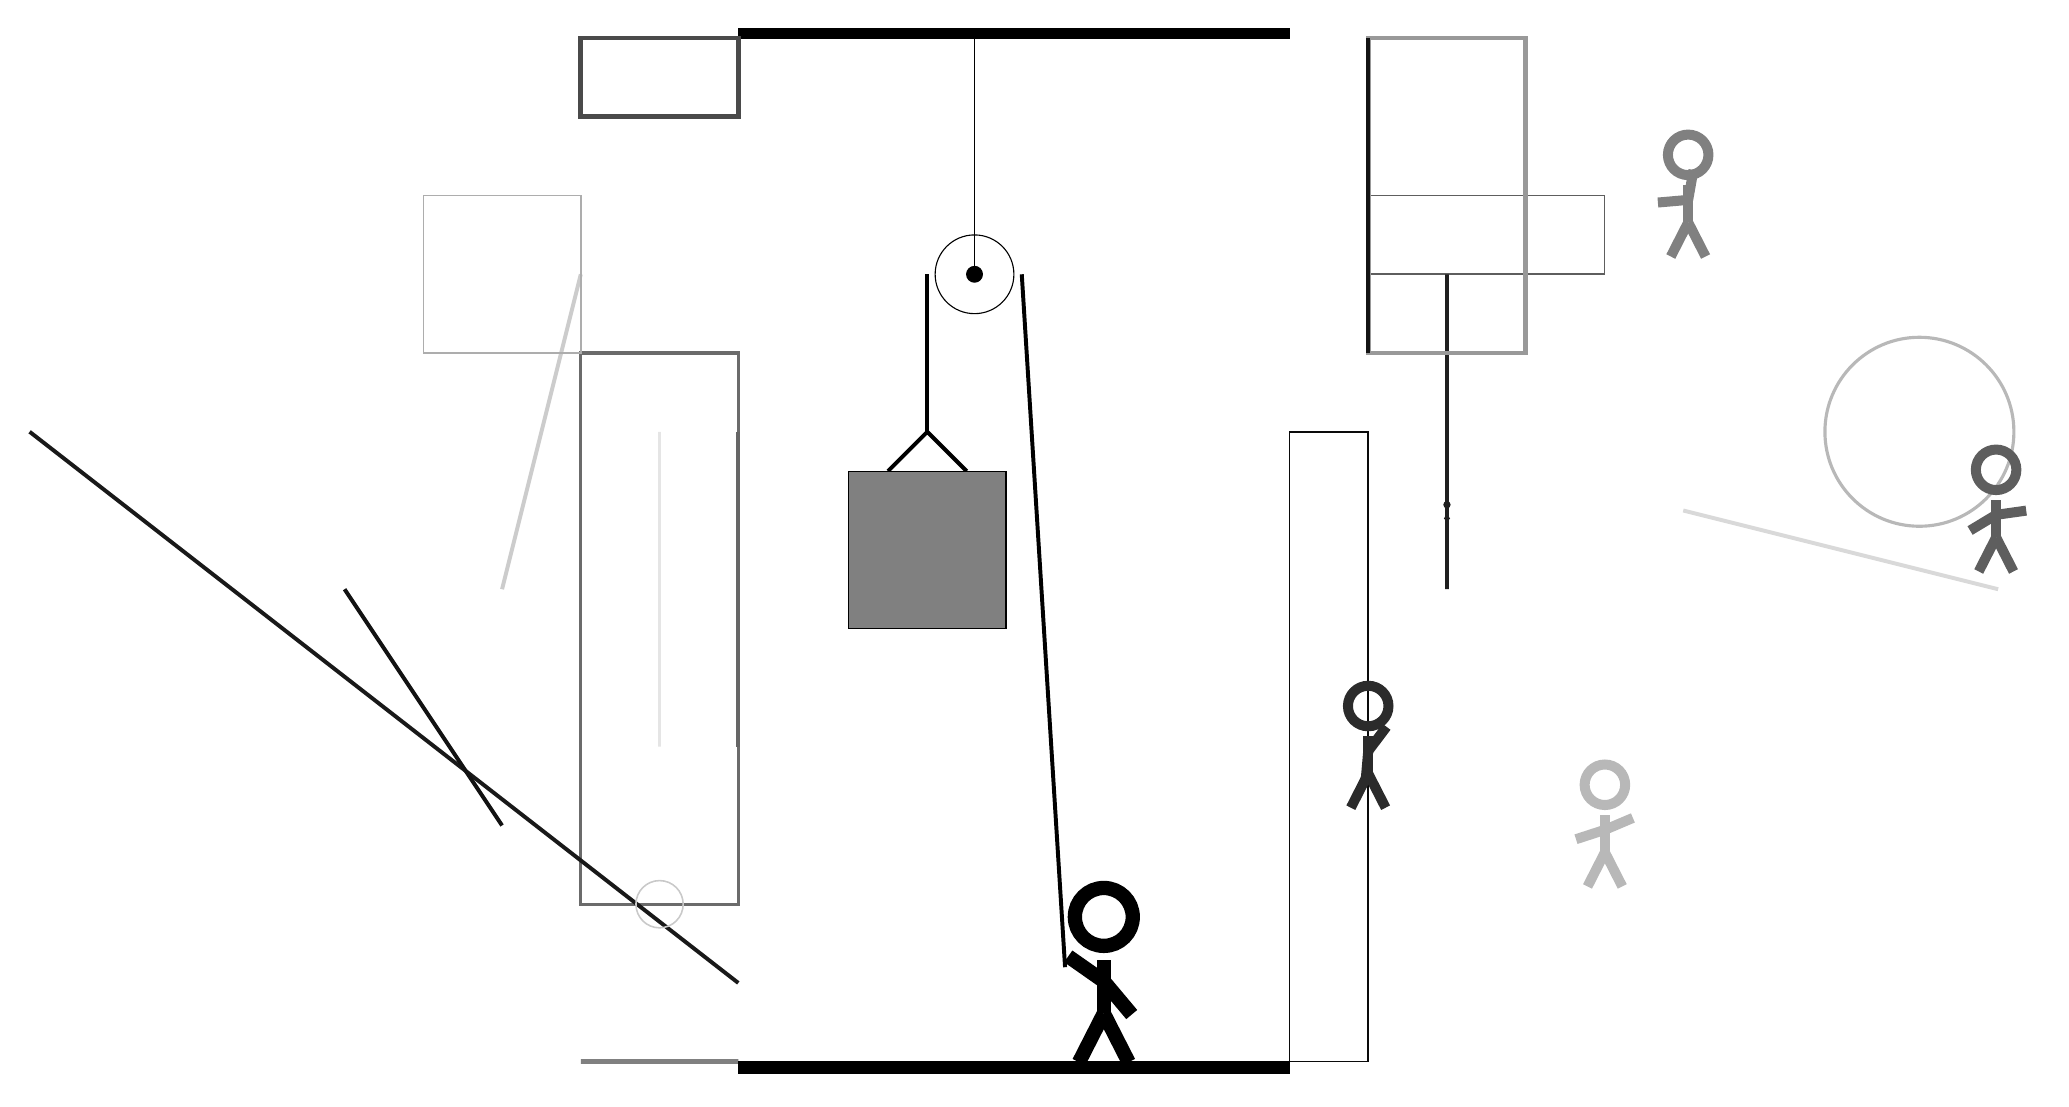
\begin{tikzpicture}
		%%%%% START %%%%%
		
		\draw[fill=black] (-2, 10) rectangle (5, 10.125);
		
		\draw (1, 7) circle (0.5);
		\draw[fill=black] (1, 7) circle (0.1);
		\draw (1, 10) -- (1, 7);
		
		\draw[line width=0.5mm] (-0.1, 4.5) -- (0.4, 5.0) -- (0.9, 4.5);
		\draw[fill=black!50] (-0.6, 4.5) rectangle (1.4, 2.5);
		
		\draw[line width=0.5mm] (0.4, 7) -- (0.4, 5.0);
		\centerarc[line width=0.5mm](1, 7)(0:180:0.6);
		\draw[line width=0.5mm](1.6, 7) -- (2.15, -1.8);
		
		\node at (2.6, -1.9) {\Strichmaxerl[10][-35][-50]};
		
		\draw[line width=0.7mm, color=black!50] (-2, -3) rectangle (-4, -3);
		
		\draw[line width=0.4mm, color=black!58] (-4, -1) rectangle (-2, 6);
		\node[line width=0.4mm, color=black!28] at (9, 0) {\Strichmaxerl[7][18][23]};
		\draw [line width=0.4mm, color=black!28](13, 5) circle (1.2);
		\node[line width=0.6mm, color=black!89] at (7, 4) {\Strichmaxerl[1][76][85]};
		\draw[line width=0.2mm, color=black!63] (6, 8) rectangle (9, 7);
		\draw[line width=0.4mm, color=black!10] (-3, 5) rectangle (-3, 1);
		
		\node[line width=0.2mm, color=black!63] at (14, 4) {\Strichmaxerl[7][31][8]};
		\draw[line width=0.5mm, color=black!20](-5, 3) -- (-4, 7);
		\draw[line width=0.5mm, color=black!90](-2, -2) -- (-11, 5);
		
		\draw[line width=0.6mm, color=black!88] (7, 3) rectangle (7, 7);
		\draw[line width=0.2mm, color=black!32] (-4, 8) rectangle (-6, 6);
		\node[line width=0.5mm, color=black!50] at (10, 8) {\Strichmaxerl[7][5][80]};
		\draw[line width=0.2mm, color=black!96] (5, 5) rectangle (6, -3);
		\draw[line width=0.5mm, color=black!15](10, 4) -- (14, 3);
		\draw[line width=0.5mm, color=black!93](-5, 0) -- (-7, 3);
		
		\draw [line width=0.2mm, color=black!21](-3, -1) circle (0.3);
		\draw[line width=0.6mm, color=black!40] (6, 6) rectangle (8, 10);
		\draw[line width=0.5mm, color=black!60](-2, 5) -- (-2, 1);
		\draw[line width=0.5mm, color=black!92](6, 10) -- (6, 6);
		\draw[line width=0.6mm, color=black!71] (-2, 10) rectangle (-4, 9);
		\node[line width=0.2mm, color=black!83] at (6, 1) {\Strichmaxerl[7][85][53]};
		
		
		\draw[fill=black] (-2, -3) rectangle (5, -3.15);
		
		%%%%% END %%%%%
	\end{tikzpicture}
\end{document}